\chapter{Results}
\label{chapter:results}

In this chapter, we present the results from the preliminary evaluation, based on the collected data (see \autoref{table:data}), the results from the semi-structured interviews, and the findings from the two questionnaires. First, we examined overall usability in \autoref{section:usability} and show high usability scores. Second, we identified two challenges when working remotely, namely a lack of mood awareness and social contacts, highlighting the need for a mood-based micro-blogging approach (see \autoref{section:lack_of_awareness_and_social_contacts}). We discuss the impact of each feature of AmbientTeams in \autoref{section:moods_were_shared_the_most}. Results show that sharing moods was the most frequently used feature. 

We observed that many participants are hesitant to share negative moods and discuss possible reasons for this in \autoref{section:negative_moods_and_honesty}. Regarding broader effects of AmbientTeams, we found that AmbientTeams 1) could increase awareness of availability and mood (\autoref{section:availability_and_mood}), 2) made it easier to get to know each other (\autoref{section:getting_to_know_each_other_better}), and 3) encouraged more (\enquote{natural}) communication in other tools (\autoref{section:bringing_back_natural_communication}). Additionally, self-reflection on moods was perceived as a positive side effect and is discussed in \autoref{section:mood_awareness_via_selfreflection}. Last but not least, in \autoref{section:workplace_isolation} we present the potential finding that AmbientTeams could potentially improve feelings of isolation in the workplace. However, as with all other findings, a more extensive study would be needed to make more meaningful statements.

Last, we analyzed the usage of AmbientTeams in \autoref{section:tool_usage_and_workflows}. Results show that AmbientTeams ran on average more than 7 hours per day (in the background) on participants' computers, with the time spent using the ambient window falling short of our expectations. Reasons for this were problems with positioning and resizing the ambient window.

\section{Lack of Awareness and Social Contacts (RQ1)}
\label{section:lack_of_awareness_and_social_contacts}
From the interviews, we identified two reasons why there is a need for mood sharing in the workplace: the lack of 1) awareness and 2) social interactions in remote work environments.

\bigskip\noindent\textbf{Lack of Mood Awareness}

\medskip\noindent P2 stated that there is a lack of awareness of the \textit{real} mood when working remotely. Even though one can see their colleagues during video conferences, there is an impression that the feelings expressed by such calls may not be real.

\begin{displayquote}
    I think it's a good idea, especially now if you work either hybrid or completely remote, I think then it is quite difficult to see the mood of your team colleagues, because now in most video conferences you make a happy face into the camera, so it is also difficult to see your mood how your mood really is right now. -P2
\end{displayquote}

To further emphasize this point, four out of five participants stated in the pre-study questionnaire that they were not or only partially aware of their colleagues' moods. According to P3, this is due to a lack of cues resulting from working from home:

\begin{displayquote}
    I like to ask people how they feel but being in a room with your colleagues gives you more information about how someone is actually feeling. -P3
\end{displayquote}

These two statements above both talk about the concept of honesty when it comes to feelings, a topic that, contrary to expectations, was talked about a lot during the interviews and is therefore discussed in more detail in \autoref{section:negative_moods_and_honesty}.

Confirming what has been mentioned in the related work (\autocite{grant2013exploration, kuwabara2002connectedness}), P4 states that being aware of your co-workers' feelings is important for personal relationships; something P4 says is important:

\begin{displayquote}
    Yes, it [feeling of co-workers] is important to me because if you think about how much time you spend with your co-workers, it is very important that you have good personal relationships with those people. -P4
\end{displayquote}

In addition, by sharing moods and states, certain conclusions can be drawn about the current workload of employees, which facilitates task assignment. Interestingly, the same participant talked about the usefulness of a state \enquote{bored}, a mood that is not currently part of AmbientTeams. However, such a mood could be a promising addition to the current selection. Before doing that, the potential implications of sharing a negative mood should be considered, something that we discuss in more detail in \autoref{section:negative_moods_and_honesty}.

\begin{displayquote}
    Sometimes I then [at a previous company] got the feedback that they already finished with work or that they have no more tasks left. With something like AmbientTeams they could set like a bored state, and I would have been able to give them a new task. -P2
\end{displayquote}

\bigskip\noindent\textbf{Lack of Social Contacts}

\medskip\noindent One participant (P1) talked about how remote working is often very task-oriented, which leads to forgetting the \textit{social aspects of an enterprise}. P3 mentioned that communication is often very business-oriented when working remotely, so conversations are usually started for business reasons only:

\begin{displayquote}
    I think during corona, you don't really have that breakroom time, so if you call somebody, it's mostly about business and not about private stuff. So, I think it's very difficult to get into a deeper connection with people you don't see that often. -P3
\end{displayquote}

In conclusion, there appears to be a need for an approach that provides mood awareness and fosters more social contacts. The following sections examine how our approach, AmbientTeams, performed in addressing the above challenges.

\section{Moods Were Shared the Most (RQ2)}
\label{section:moods_were_shared_the_most}
Moods were the most actively shared statuses, with a total of 31 moods shared (out of 45 total interactions). According to the interviews, a primary reason for sharing moods was the automatically scheduled popup, which helped to remind the participants to share something. The data confirm this finding; 25 of the 32 shared moods were shared through the scheduled popup window. However, the participants usually just shared the mood through an emoticon and did not attach a text message, as shown in \autoref{fig:moods_status_messages}. From P2, we learned that a potential reason could be that it was simply a lot quicker only to share the mood via emoticon, requiring only one click. P5 also mentioned that he/she did not see a reason to provide any more information about the shared moods (which was \enquote{tired} ten out of 12 times).

\begin{figure}[h]
    \centering
    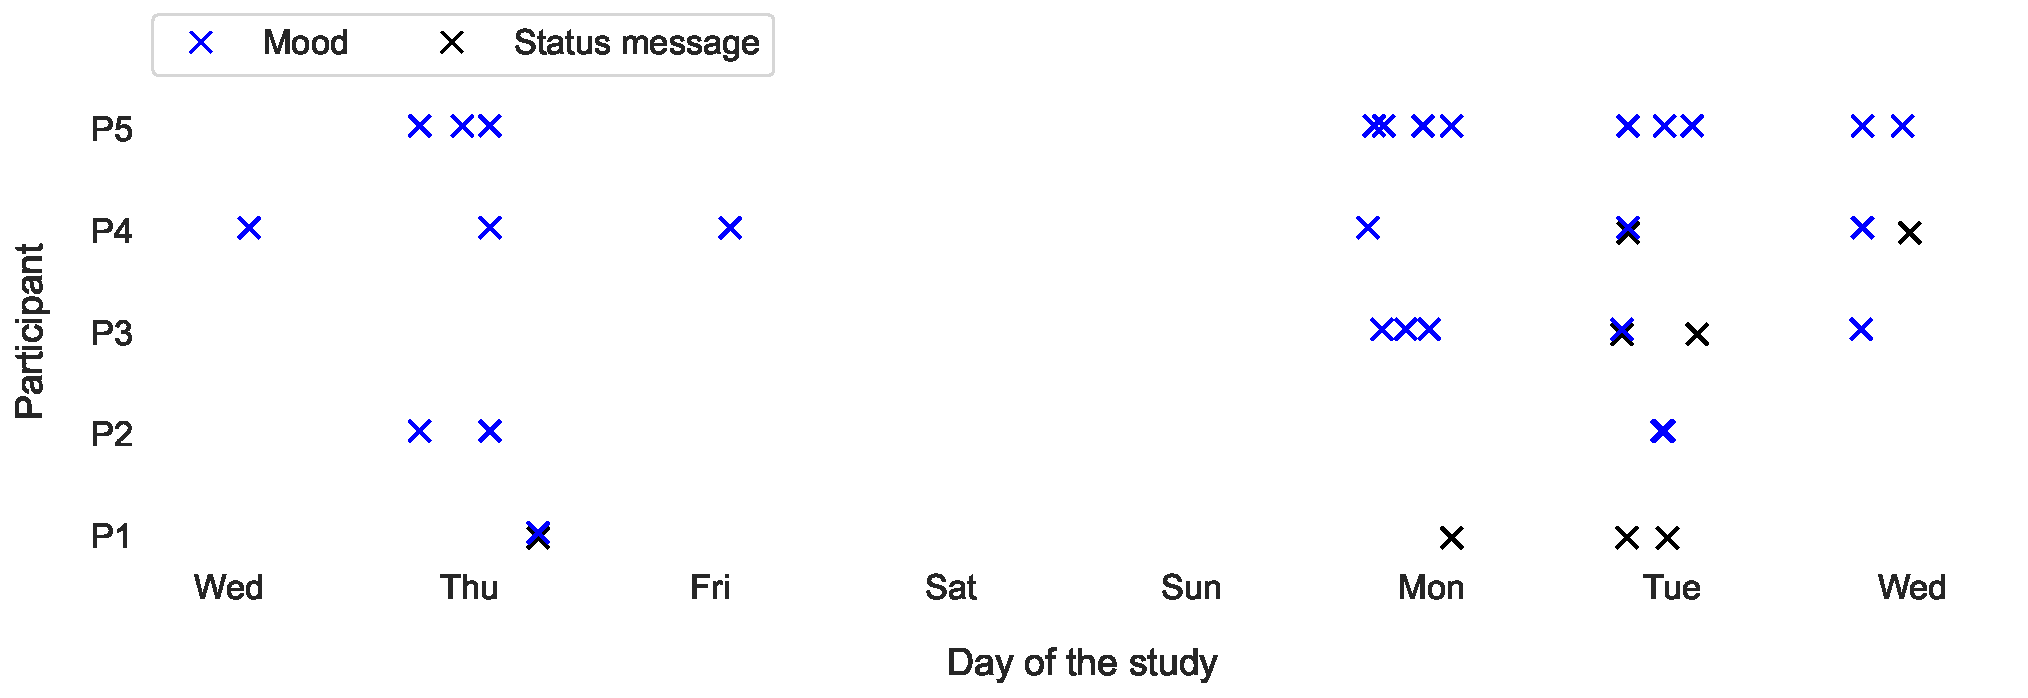
\includegraphics[width=\linewidth]{plots/moods_status_messages.pdf}
    \caption{Moods and Status Messages Shared}
    \label{fig:moods_status_messages}
\end{figure}

% \begin{displayquote}
%     If we were not in a test phase, maybe I would not share that much if I saw that the others are also not really sharing anything. \\
%     -P3
% \end{displayquote}

In contrast to the commonly shared moods, only eight status messages were shared. The contents of all status messages can be seen in \autoref{table:status_messages}. In general, none of the status messages contained any work-related information.

\begin{table}[h] \footnotesize
    \centering
    \begin{tabularx}{.8\textwidth}{l l l l l}
        \toprule
        ID & Participant & Day \& time & Status message            & Attached mood \\
        \midrule
        1  & P1          & Thu, 20:50  & Hiiii                     & Happy         \\
        2  & P1          & Mon, 16:00  & Hiiii                     & -             \\
        3  & P3          & Tue, 09:00  & Hopp Schwiiiiiiz!         & Love          \\
        4  & P1          & Tue, 09:30  & Switzerland!!!            & -             \\
        5  & P4          & Tue, 09:37  & Feeling bad for Mbappé :( & Neutral       \\
        6  & P1          & Tue, 13:32  & Hey how are you?          & -             \\
        7  & P3          & Tue, 16:30  & nznznznz, still vibin'    & -             \\
        8  & P4          & Wed, 13:42  & How is life?              & -             \\
        \bottomrule
    \end{tabularx}
    \caption{Status Messages Shared and the Moods Linked to Them}
    \label{table:status_messages}
\end{table}

Looking at \autoref{fig:moods_status_messages} or \autoref{table:status_messages} shows that in only three cases, moods and status messages were shared simultaneously. To our surprise, no negative moods (such as \enquote{tired}, \enquote{angry}, or \enquote{sad}) were further explained with the help of a status message. All three attached moods were either of a happy or neutral nature. However, the neutral mood shared with status message 5 (despite its sad tone) could be due to the absence of an empathy mood in AmbientTeams or a possible mistake by that participant. It becomes apparent that 62.5\% of all status messages were sent on one day. The first three messages on that day were all related to a soccer game, which seemed to be of general interest to the group. P3 also described the motivation for sharing such common feelings:

\begin{displayquote}[][]
    [...] if you have something that you are very happy about, you think that other people also share, then you are more motivated to share it as well. -P3
\end{displayquote}

While the scheduled popup window helped remind participants to share something, knowing the importance of social interactions with colleagues (P1) or feeling closer to each other (P5) were other motivators for sharing something with the team.

Given the relatively short time of the study, it is not surprising that many of its features have not been used. Specifically, the features aimed at spontaneous interactions, such as the breakroom and random pairing for a video call, were not used at all. There were two attempts to set up a breakroom, one on the second day of the study and one on the second to last day, but neither was successful because no other team member joined. During the interview P3 provided a possible explanation for why the spontaneous video chat features were not used:

\begin{displayquote}[][]
    [...] I have to mention that two or three weeks ago we started with virtual breakrooms on Friday afternoons to try to keep up with people from work, especially for new people, because we don't really get the chance to get to know each other in home office. -P3
\end{displayquote}

Consequently, it is possible that it was sufficient for the participating teams to meet once a week in their own virtual breakroom. Like the breakroom, the direct video calls and nudging functionality were only used for testing purposes during the first kick-off meeting. %While this shows that the team was aware of how to use these features, they do not seem to have felt the need to do so.

The picture is somewhat different when analyzing the direct messages that were sent via AmbientTeams. A total of six direct messages were sent through AmbientTeams, from three different participants. One of these direct messages was a response to a missed call (during the kick-off meeting), and the other five were either a greeting or of the type \enquote{what are you doing?}. P1 gives an indication of why the team did not use the functionality described above:

\begin{displayquote}
    Because now it's a bit, you know I can write to somebody in Microsoft Teams or AmbientTeams, and I would normally pick MS Teams because we use it, and you also have a message history which you don't have in AmbientTeams. -P1
\end{displayquote}

Essentially, P1 explains that AmbientTeams needs to differentiate itself from MS Teams, and it does so with the \enquote{Twitter} approach to broadcasting moods and status messages, but not so much with other communications functionality.

\section{Negative Moods and Honesty (RQ2)}
\label{section:negative_moods_and_honesty}

Looking at \autoref{fig:moods_distribution}, it is clear that except P5, who mostly shared the mood \enquote{Tired}, the most frequently shared moods were positive (especially \enquote{Happy}).

\begin{figure}[h]
    \centering
    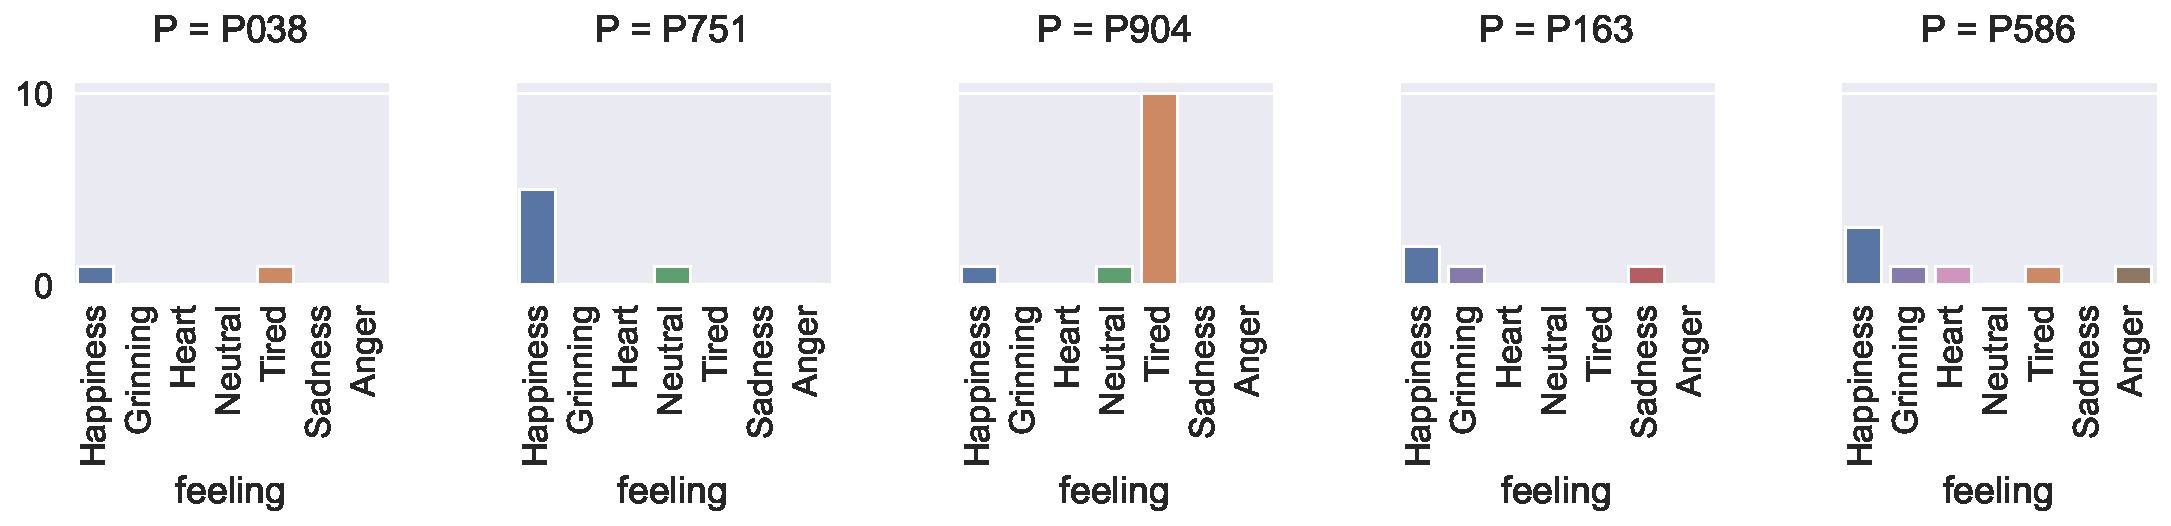
\includegraphics[width=\linewidth]{plots/moods_distribution.pdf}
    \caption{Distribution of Shared Moods}
    \label{fig:moods_distribution}
\end{figure}

Therefore, this finding raised the question of whether this was the true distribution of moods during the study or whether there might be a tendency for more positive moods to be shared, regardless of their true feeling. While P1 sees no problem with sharing negative moods \textit{\enquote{we are not in a happy boat where everyone is happy all the time}}, others (P2, P3, P4) would be more hesitant to share such moods. Reasons for not sharing negative moods include 1) \textit{not wanting to explain further}, either for personal reasons or to avoid being distracted (P2), 2) \textit{being fairly new to the company}, 3) \textit{not wanting to share with the whole team} (P3), or 4) because \textit{no one wants to talk about negative feelings at work}.

% \begin{displayquote}
%     Yes, I think then it would be harder to share an angry mood. And if you are mad for private reasons, you maybe don't want to explain more. \\
%     -P2
% \end{displayquote}

% \begin{displayquote}
%     I would not share those things, like when I am tired or angry. \\
%     -P3
% \end{displayquote}

P4 further differentiated between the severity of moods experienced, indicating that regular, daily negative moods may not benefit colleagues, so stronger negative moods are more likely to be shared:

\begin{displayquote}
    I don't think I would share regular negative moods when having a bad day, for instance, being this new to a company. If something really severe were to happen, however, let's say something personal or family-related, I would share such moods to inform other people. -P4
\end{displayquote}

While most participants seem hesitant about sharing negative moods, P2 mentioned several times during the interview that in cases where a colleague would share a negative mood, P2 would try to help that person.

P4 also brings up that sharing positive moods, even if they are not truthful, could positively affect the person sharing:

\begin{displayquote}
    Sharing something \enquote{fake} positive could potentially make them feel better. -P4
\end{displayquote}

% \begin{displayquote}
%     But I always said that at this time that I had a good mood, this time this was honest, but I am not sure whether I would also share it if one day I had a bad mood. I am not sure if I then would be that honest to share it then directly online. \\
%     -P2
% \end{displayquote}

% -> Potentially undesired interruptions

% \begin{displayquote}
%     First reason is if I make, for example, an angry or sad mood, then everyone would text me, and I think I will maybe lose my focus because they would ask me why I was feeling in this way etc. And I think the second reason is that in the online world it is a lot easier to hide bad feelings, and you try to present yourself in the best way. \\
%     -P2
% \end{displayquote}

% \begin{displayquote}
%     It's easier to share positive feelings within a working environment compared to negative feelings because nobody wants to talk about negative feelings. \\
%     -P3
% \end{displayquote}

% While P3 also claims that talking about feelings is very important, sharing such personal information is not something that he/she likes to do.

% \begin{displayquote}
%     I mean of course it is very important that you talk about these kinds of things [feelings], but you don't want to share it with the whole team. \\
%     -P3
% \end{displayquote}


\section{Tool Usage and Workflows (RQ3)}
\label{section:tool_usage_and_workflows}

\subsection{Ambient and Overview Window}
\autoref{fig:opened_vs_focused} shows that both the ambient window and the team overview window were open almost exclusively when these windows were in focus. In other words, these two windows were opened, an interaction occurred, and then they were closed or minimized again, disappearing from the user's screen. This is the result we expected in the case of the team overview. However, contrary to our assumptions, the ambient window was used in a very similar way. Conclusively, the ambient window was rarely kept open as a glanceable, always-on-top team view when working on other tasks.

\begin{figure}[h]
    \centering
    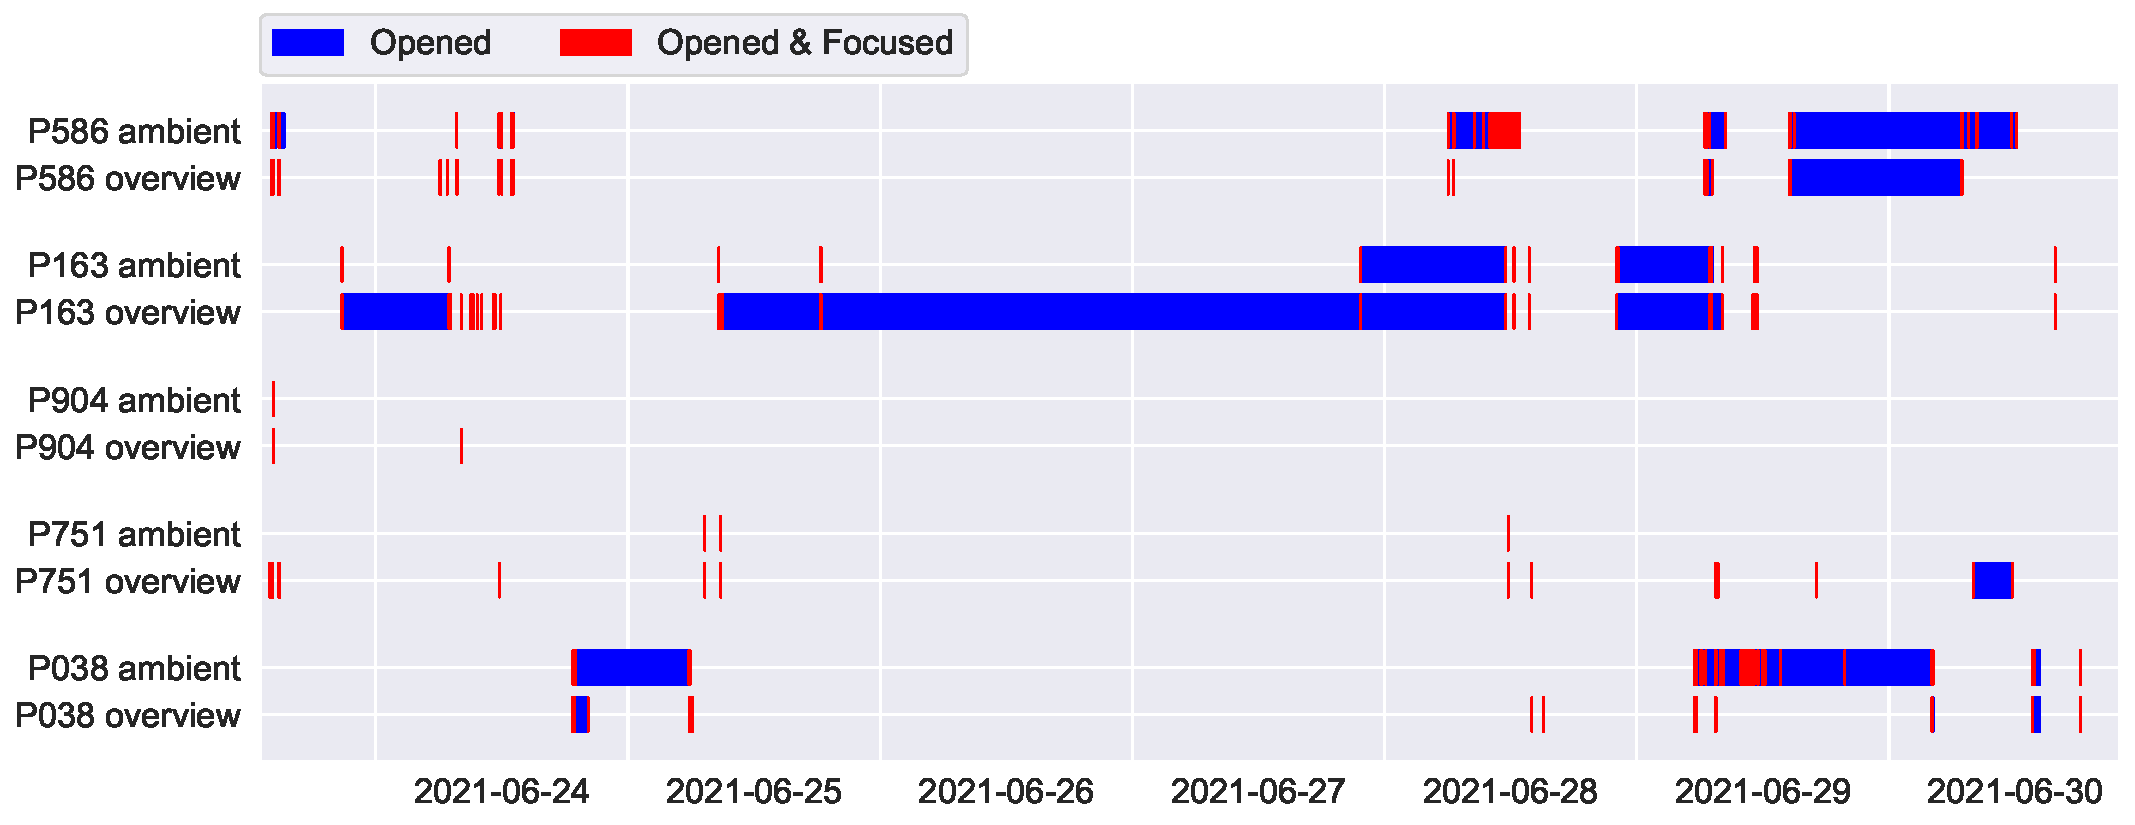
\includegraphics[width=\linewidth]{plots/open_vs_focus.pdf}
    \caption{Time Using AmbientTeams: Opened vs. Opened and Focused}
    \label{fig:opened_vs_focused}
\end{figure}

The interviews gave us some more insights into possible reasons for why the ambient window was not kept open while working on other tasks.

\begin{displayquote}
    I tried it in the corner of the monitor, then it did not work, but in the corner of the window did not really work because there you have to click to close other windows. Then I put it somewhere in the middle, but then I needed to put some buttons there, so sometimes I got annoyed and then closed it. -P1
\end{displayquote}

We suspect that this user was using a single monitor configuration and thus had difficulty finding a suitable position for the ambient window. P3 mentioned that the ambient window was too small and, therefore, difficult to move. This suggests that this participant might have missed the introduction of the resizing feature during the kick-off meeting, or the part was not demonstrated in enough detail. In addition to the inconvenience of the ambient window perceived by P1 and P3, P2 mentioned that manually closing an application that launches automatically is almost automatic for them due to established habits. The inconvenience and difficulty of positioning the ambient window is a fairly crucial issue that may require further development of AmbientTeams; the case described by P2 could be resolved in a future study by not allowing the closing of the ambient window.

To better fit the ambient window into the workflow, P1 suggested that ideally, it should not remain on top of other windows. Instead, it should disappear into the background and only come back to the foreground when a team member has shared something new. P3 also suggested that the ambient window should ideally be hidden when not in use.

Despite the criticism of the ambient window, it was used by all participants except P5 and was seen by P4 as one of the best aspects of AmbientTeams due to its refreshing look and feel:

\begin{displayquote}
    I liked that the ambient window feels very dynamic and refreshing compared to other tools. -P4
\end{displayquote}

Despite this positive statement, this participant used the team overview window more, which is surprising since all participants were only part of one team during the study, which we believe eliminates the potential advantage of the team overview window. 

\subsection{Usability}
\label{section:usability}
%  more info on usability score: https://measuringu.com/sus/
% A SUS score above 68 would be considered above average, and anything below 68 is below average.
% # A SUS score of 74 has higher perceived usability than 70\% of all products tested. It can be interpreted as a grade of a B-.
While there were no usability issues during the study, we still asked the participants to fill out a usability questionnaire before the final interview. The results from the standardized usability questionnaire that participants answered at the end of the study are presented in \autoref{fig:usability_questionnaire}. For the questions with even numbers, e.g., Q2, Q4, etc., negative (red) answers are desirable, while for questions with odd numbers, e.g., Q1, Q3, etc., positive (blue) answers are ideal. In general, the results look very promising, showing high usability ratings overall. However, there are some answers that are worth discussing. The \enquote{disagree} answer from Q1 came from P3. This participant also did not think that the various features of the application were well-integrated (Q5). The reason for these answers could be found in the interview, where the following statement was made:

\begin{displayquote}
    Uhm, as a separate tool, I would not use it. Integrated into another communication tool, I might use it, yes. -P3
\end{displayquote}

The \enquote{agree} response in questions Q4 and Q10 came from P2, indicating that the number of features in AmbientTeams is quite challenging to understand on the first encounter. Nevertheless, this participant did not mention any usability issues either in the interview or through direct feedback, leading us to believe that the application was easy to use after the initial challenge of understanding the application.

\begin{figure}[h]
    \centering
    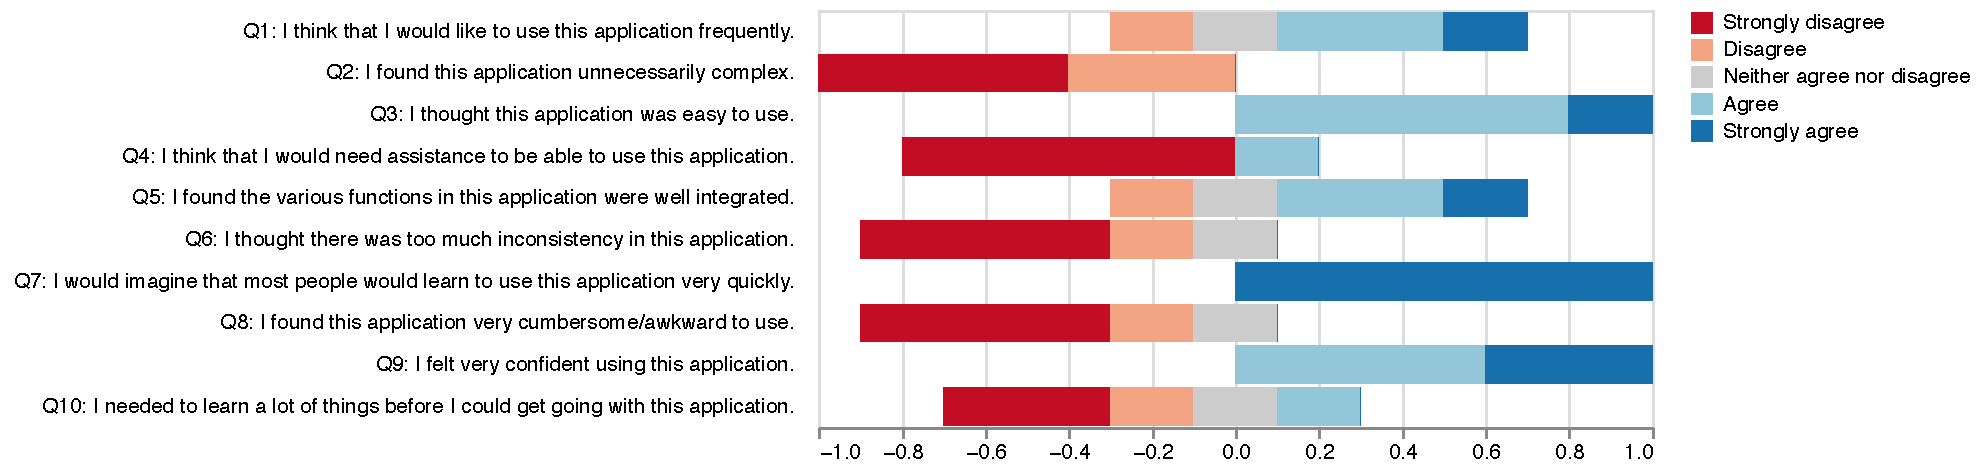
\includegraphics[width=\linewidth]{plots/usability_likert.pdf}
    \caption{Usability Questionnaire Results}
    \label{fig:usability_questionnaire}
\end{figure}

Following the instructions from \textcite{sauroSUS}, each participant's responses were then converted into the SUS score to obtain a comparable value. The resulting average SUS score was 81.1 ($\sigma=6.58$, $min=70.0$, $max=90.5$) across all five participants. According to \textcite{sauroSUS}, one would need to score above 80.3 to be in the top 10\% of the 500 studies using the SUS. 80.3 is also the point where users are more likely to be recommending the product to a friend \autocite{sauroSUS}, showing that AmbientTeams was easy and intuitive to use.

%\begin{table}[h] \footnotesize
%    \centering
  %  \begin{tabularx}{.35\textwidth}{X X}
  %      \toprule
  %      Participant & SUS score \\
  %      \midrule
  %      P1          & 82.5      \\
  %      % \hline
  %      P2          & 80.0      \\
  %      % \hline
  %      P3          & 70.0      \\
  %      % \hline
  %      P4          & 82.5      \\
  %      % \hline
  %      P5          & 90.5      \\
  %      \midrule
  %      Average     & 81.1      \\
  %      \bottomrule
  %  \end{tabularx}
 %   \caption{Usability Questionnaire Results and Resulting SUS Score}
%    \label{table:sus}
%\end{table}


\subsection{Availability}
A detailed timeline view of participants and their selected availability state (\enquote{Available}, \enquote{Focused}, or \enquote{Happy to Interact}) during the study is visualized in \autoref{fig:non_offline}. The time a user is in one of these three states is considered the time the application was running. This time also includes the period when the application was not active and was running in the background. This is possible because the user is automatically put into an offline state when the connection to the server is lost. Upon successful reconnection to the server, the user's availability state is also automatically set to \enquote{Available}. It is, therefore, possible that this metric could be slightly flawed if users manually set their availability status to \enquote{Offline}. However, this would only underestimate the online time displayed in \autoref{fig:non_offline}. Thus, the times shown there are conservative. Apart from inactivity on weekends, five out of a total of 30 working days showed no or minimal runtime (less than one hour), leading us to remove those five data points. The average time spent in an online state, and thus running AmbientTeams, was 7.68 ($\sigma=3.09$) hours per day, with a minimum of 2.04 and a maximum of 12.7 hours. The fact that P1 could not attend the kick-off meeting with the rest of the group explains the lack of use on the first day of the study. In general, the relatively short runtime on the first day was to be expected since the kick-off meeting was held in the early afternoon. The remaining days with very short runtimes most likely indicate non-work days for these participants. This is because, if those were workdays, AmbientTeams would have started automatically as soon as the computer booted up.

\begin{figure}[h]
    \centering
    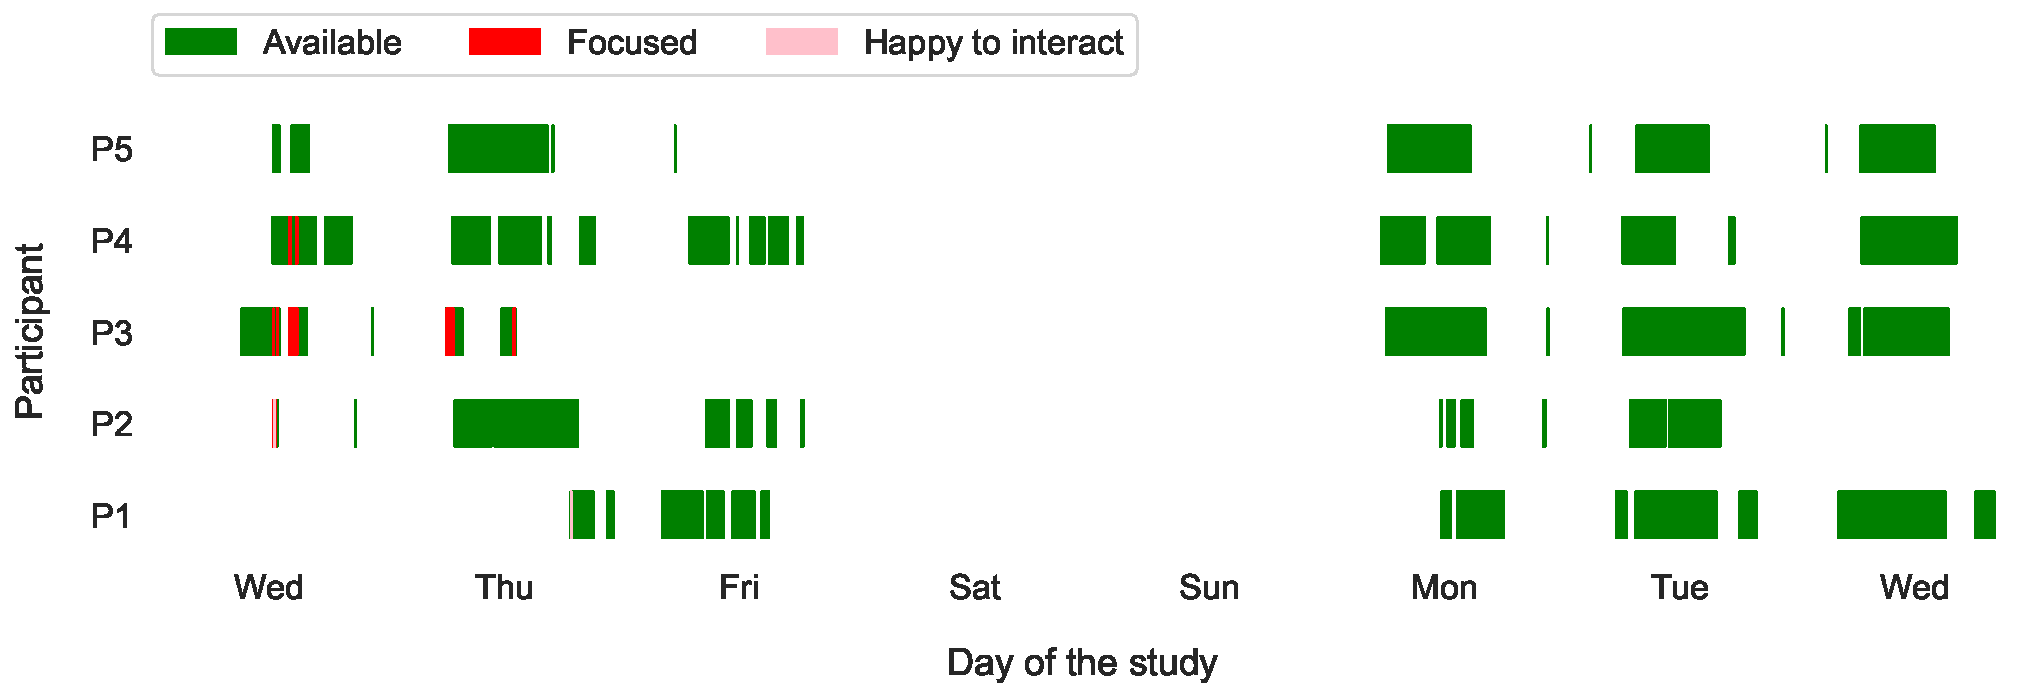
\includegraphics[width=\linewidth]{plots/non_offline.pdf}
    \caption{Time Spent In the Different Availability States}
    \label{fig:non_offline}
\end{figure}

The results show that participants did not change their availability state often and thus relied mainly on AmbientTeams' automatic setting of the availability state. The \enquote{Focused} availability state was selected a few times in the first two days of the study, but this behavior did not continue throughout the study. Similarly, P1 and P2 selected the \enquote{Happy to Interact} availability state a total of three times. However, two of those lasted for two seconds, and one during the kick-off meeting for only one minute, making it barely visible in \autoref{fig:non_offline}.

\section{Availability and Mood (RQ4.1)}
\label{section:availability_and_mood}
The first effect of AmbientTeams was that participants learned who was around (P1, P3) and how they were doing (P1, P4). P5 also noted a significant difference from their previous way of sharing moods and feelings, which was usually via text in the morning:

% \begin{displayquote}
%     Also, sometimes for just checking who is online and who is grayed out. -P3
% \end{displayquote}

\begin{displayquote}[][]
    [...] I wouldn't have known how you were doing during the day without AmbientTeams. [...] And, I think that's when you get additional information about how you're doing during the day. -P5
\end{displayquote}

AmbientTeams helped P4 raise awareness of colleagues with whom they otherwise have little or no regular communication:

\begin{displayquote}
    I think it was very interesting to see moods and states of team members with whom I might not be currently working together too closely. -P4
\end{displayquote}

This increased awareness had other implications, namely the opportunity to get to know each other better and to bring back a more natural way of communicating in remote work. We will discuss both in the next sections.

\section{Getting to Know Each Other Better (RQ4)}
\label{section:getting_to_know_each_other_better}
AmbientTeams led one person in particular (P4) to find out that a colleague was very funny, which was unknown to this person before the study.

\begin{displayquote}
    Yes, actually about one particular person in the team. I did not know that this person was so funny before using AmbientTeams. The fact that I got to know one person a lot better during this one week and also having non-work-related talks now already exceeds my expectations for the study, to be honest. -P4
\end{displayquote}

It is no surprise that P4 was pretty new to the company and thus did not have the chance to get to know all the team members too well. Due to this, this participant liked the fact that \textit{\enquote{this feature [mood sharing] allows to discover more about your colleagues, and it sheds light into a part that we tend to keep only for ourselves}}, in particular seeing \textit{\enquote{moods and states of team members with whom I might not be currently working together too closely}}.  While not learning something completely new, P3 mentioned that using AmbientTeams confirmed the previous assumption that \textit{\enquote{one team member is really just always very positive and too nice}}, showing that there were in total two team members who took away a promising finding from the one week study.

We thus conclude that AmbientTeams has the potential to ease getting to know individual team members better, especially for new team members, and to allow learning more about team members with whom you might not be in constant exchange.

% \begin{displayquote}
%     Not really, to be honest. I just had the confirmation that one team member is really just always very positive and too nice. -P3
% \end{displayquote}

\section{Bringing Back \enquote{Natural} Communication (RQ4)}
\label{section:bringing_back_natural_communication}
This section demonstrates the capabilities of AmbientTeams to bring back the more \enquote{natural} communication known from traditional office work to a remote environment. Such communication is enabled by providing \textit{a lot more opportunities to approach another} (P5). P1 explains that by sharing moods and status messages with the entire team, everyone can see it, similar to when the entire team is in the office, and as a consequence, can react to what has been shared:

\begin{displayquote}[][]
    [...], but I actually found it if you share it with the whole team. Because sometimes people then come back to you that you don't expect. So I mean, sometimes you don't have a good mood and people see it and want to cheer you up. So this substitutes a bit that part of the office life. -P1
\end{displayquote}

Another reason for how AmbientTeams can trigger communication includes \textit{seeing when someone comes online} (P1), which resulted in contacting this person. We see this as the equivalent of going into the office and being reminded of something that needs to be done simply by seeing your co-workers. Also, the fact that the majority of the participants would not necessarily share negative moods, P2 mentioned that he/she would still offer help in cases of an angry or stressed mood, another possible communication trigger.

Although P2 indicated that AmbientTeams makes it easy to start a conversation by \textit{\enquote{simply clicking on the avatar of [a colleague] to start a conversation}} this was not observable in the data collected, as few direct messages were sent and no video calls were made. We, however, observed that AmbientTeams served as a trigger for communication with other tools (e.g., Microsoft Teams, Zoom), which was also brought up in the interviews of P4 and P1. To this end, we also analyzed participants' active window titles during the study to see if there was a higher likelihood of visiting external communication applications after leaving AmbientTeams. More details on active window titles can be found at the end of \autoref{table:data}. As you can see in \autoref{fig:active_windows} on the left, AmbientTeams was the tenth most frequently used active application. Over the entire duration of the study, the most common communication tools among all participants were Microsoft Teams (4th), Microsoft Outlook (5th), and Skype (9th). The distribution in the chart on the right includes only the active applications that immediately followed AmbientTeams' usage. Two of the three previously mentioned communication tools also improved in rank: Microsoft Teams (rank 2) and Skype (rank 6). While it is not clear whether the communication promoted by AmbientTeams was work-related or not, P4 mentioned during the interview that he/she had more non-work-related communication during the study. The fact that Microsoft Outlook was not affected and remains on rank 5, further suggests that AmbientTeams promoted communication in other tools focusing on informal communication.

\begin{figure}[h]
    \centering
    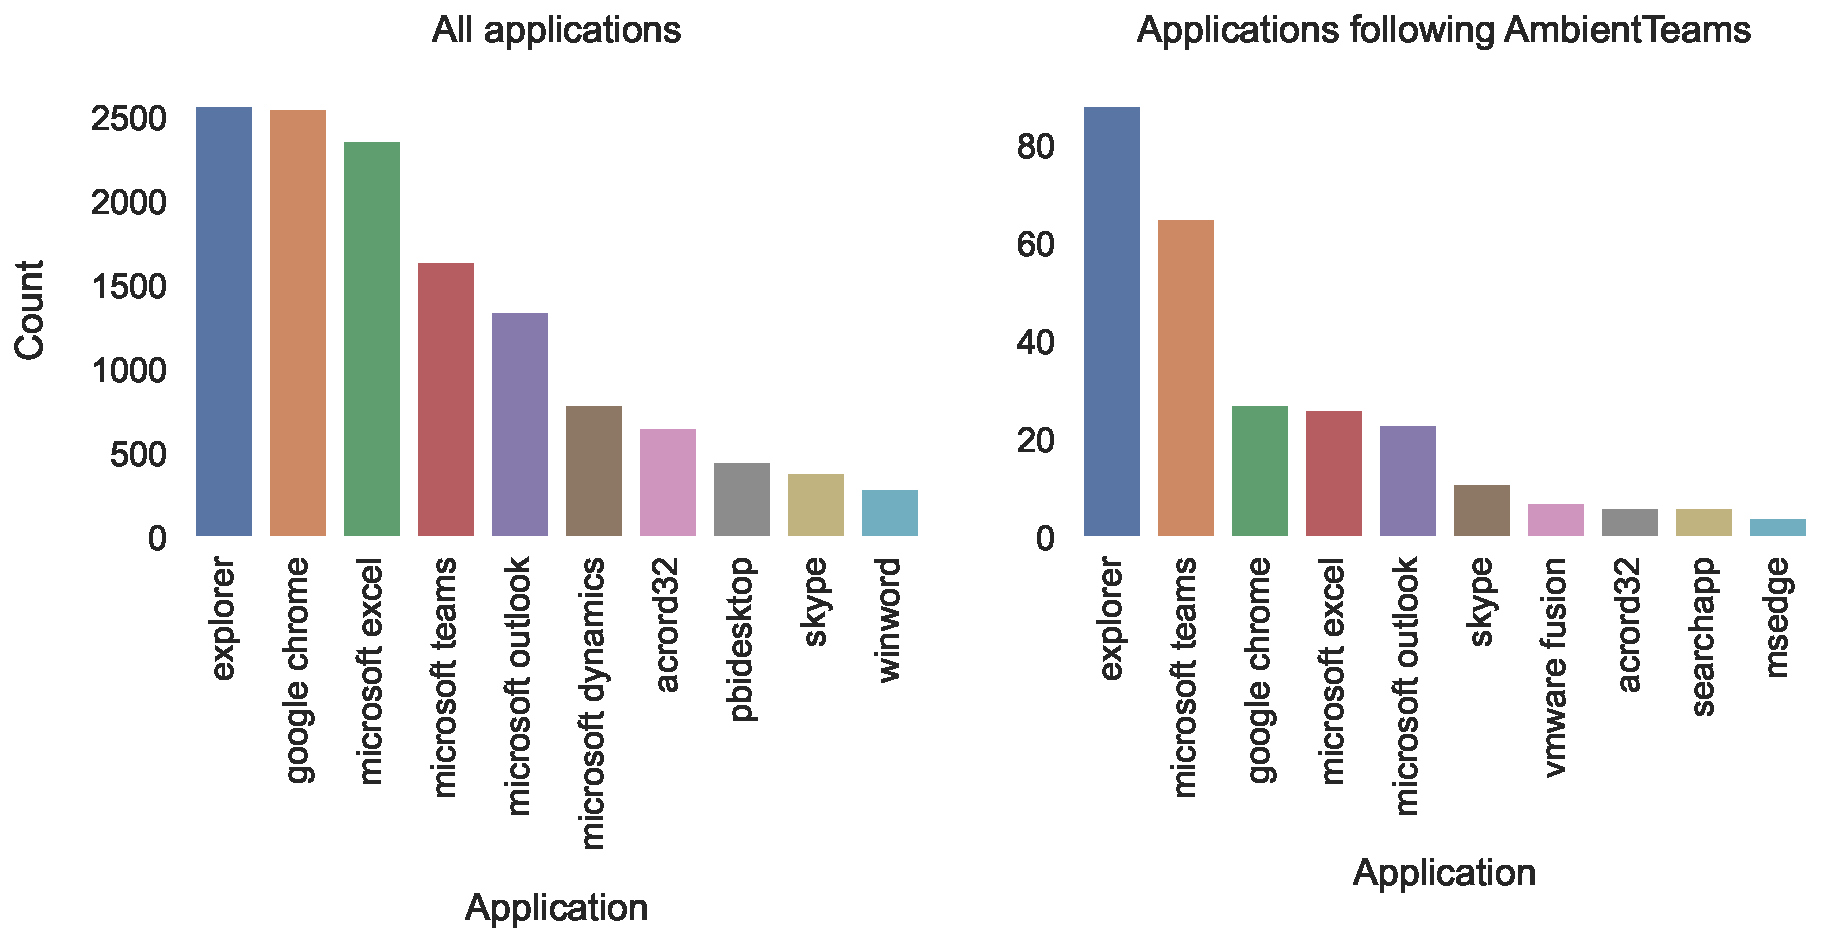
\includegraphics[width=.7\linewidth]{plots/active_windows.pdf}
    \caption{Overall Active Application Distribution and Active Applications Following AmbientTeams}
    \label{fig:active_windows}
\end{figure}


% \begin{displayquote}
%     I had more non-work-related communication, however, outside of AmbientTeams in our existing tool. -P4
% \end{displayquote}

% \begin{displayquote}
%     So, for example, I saw that somebody pushed \enquote{good morning}, then I thought \enquote{ahh okay I need to speak to this person about some topic}, so I called this person on MS Teams. -P1
% \end{displayquote}

% Reason: Lower barrier

% \begin{displayquote}
%     Yes, definitely. It provides a lot more opportunities to approach another. -P5
% \end{displayquote}

% \begin{displayquote}
%     Because if you only have to click on the avatar of Zsuzi or Adelina to start a conversation. -P2
% \end{displayquote}

% Reason: Help offering

% \begin{displayquote}
%     I think in that study not. But if somebody would have set an angry or stressed mood I would have helped him/her, if my current knowledge allowed it. -P2
% \end{displayquote}

\section{Mood Awareness via Self-Reflection (RQ4.2)}
\label{section:mood_awareness_via_selfreflection}

\begin{displayquote}
    I think it impacted myself because you're always prompted to think about your own mood. -P4
\end{displayquote}

In the previous sections, we presented results depicting the effect of AmbientTeams on other team members. However, we also found impacts on the person sharing moods themselves. More concretely, the self-reflection side of AmbientTeams was talked about by three people (P3, P4, and P5). P5 realized how their moods changed: \textit{\enquote{then maybe a few hours later you realized, I'm actually not tired or not so neutral, but rather happy}}. We argue that mood awareness via self-reflection is something that could have many more applications and benefits. During the interview, one participant even gave a concrete example of how reflecting on moods could help find potentially hidden areas of interest.

\begin{displayquote}
    If I had something that could then show me afterward that for example, every time I do something for IT I am very happy, then I can maybe try to seek more tasks in IT and find my potential in IT and my life itself to make any further education for instance. -P3
\end{displayquote}

\section{Workplace Isolation (RQ4.3)}
\label{section:workplace_isolation}

The above sections may already suggest the ability of AmbientTeams to reduce feelings of workplace isolation within knowledge work teams. This qualitative data was complemented by our approach to measure workplace isolation quantitatively; a questionnaire was surveyed before and after the study period. Before looking at the results of the questionnaires, it should be noted that we had to adjust the scale due to an error on our side. The original workplace isolation questionnaire uses a 7-point Likert scale. Unfortunately, our post-study questionnaire included a flaw where its answer range was only a 5-point Likert scale. To make the two somewhat comparable, the answers from the pre-study questionnaire for \enquote{somewhat disagree} and \enquote{disagree} were combined into \enquote{disagree}, and similarly the answers for \enquote{somewhat agree} and \enquote{agree} were combined into \enquote{agree}.

\begin{figure}[h]
    \centering
    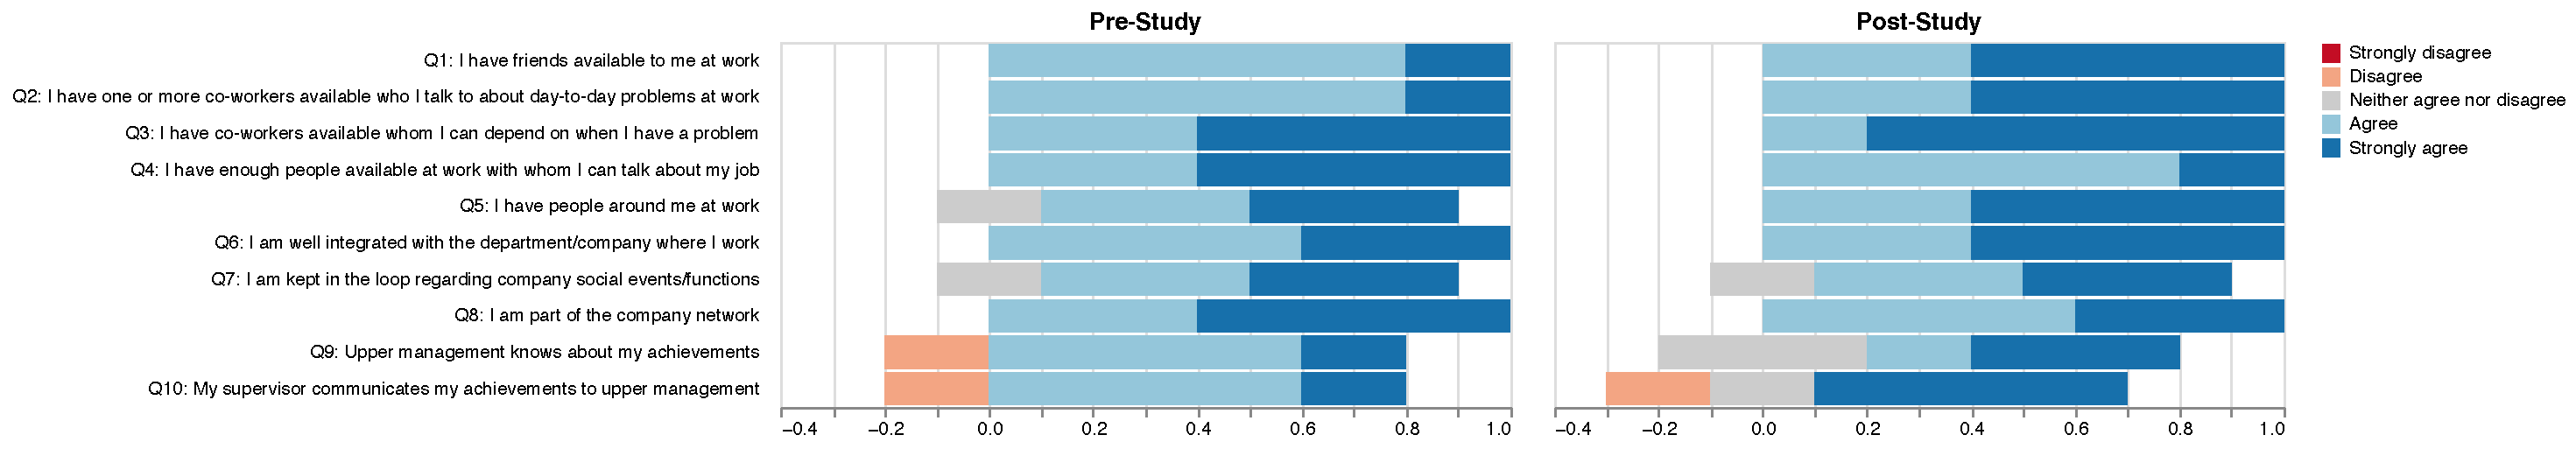
\includegraphics[width=\linewidth]{plots/workplace_isolation_likert.pdf}
    \caption{Results From the Workplace Isolation Questionnaire: Pre-Study vs. Post-Study}
    \label{fig:workplace_isolation}
\end{figure}

In \autoref{fig:workplace_isolation}, we see a slight trend toward more \enquote{strongly agree} for questions 1-3, 5, 6, 9, and 10, indicating a decrease in feelings of isolation at work. However, some responses also worsened slightly, namely Q4 and Q8. Despite the results showing improvements in Q9 and Q10, we cannot assume that these results are effects attributable to the use of AmbientTeams for two reasons. First, the content discussed within and facilitated by AmbientTeams was not work-related. Second, due to the small size of the study, there was no control group, so a comparison between the two questionnaire results is highly speculative. Nonetheless, as in this study, the questionnaire could be a suitable supplement for a more extensive study in the future to obtain more accurate information about perceptions of isolation in the workplace. We see it as a valuable complement to the semi-structured interview and are optimistic about the potential of AmbientTeams to reduce feelings of workplace isolation in knowledge work teams.

